\documentclass{ctexart}
\usepackage{geometry}
\usepackage{graphicx}
\usepackage{float}
\usepackage{minted}
\renewcommand{\contentsname}{目\ 录}
\renewcommand{\appendixname}{附录}
\renewcommand{\refname}{参考文献}
\renewcommand{\figurename}{图}
\renewcommand{\tablename}{表}
\renewcommand{\today}{\number\year 年 \number\month 月 \number\day 日}


\begin{document}


\title{\Huge 实验一}
\author{\\姓\ 名:任\ 永\ 文\\
    学\ 号: SA23011253\\\\
    强化学习\\
    (秋季, 2023)\\\\
    中国科学技术大学\\
    计算机科学与技术学院\\
}
\date{\today}
\maketitle
\newpage


\section{实验目的}
\begin{itemize}
    \item 理解、学习蒙特卡罗算法原理,并编码实现first-visit版本
    \item 理解、学习TD算法原理,并编码实现SARSA、Q-learning
\end{itemize}



\section{实验原理}
\subsection*{MC原理}
\begin{figure}[H]
    \centering
    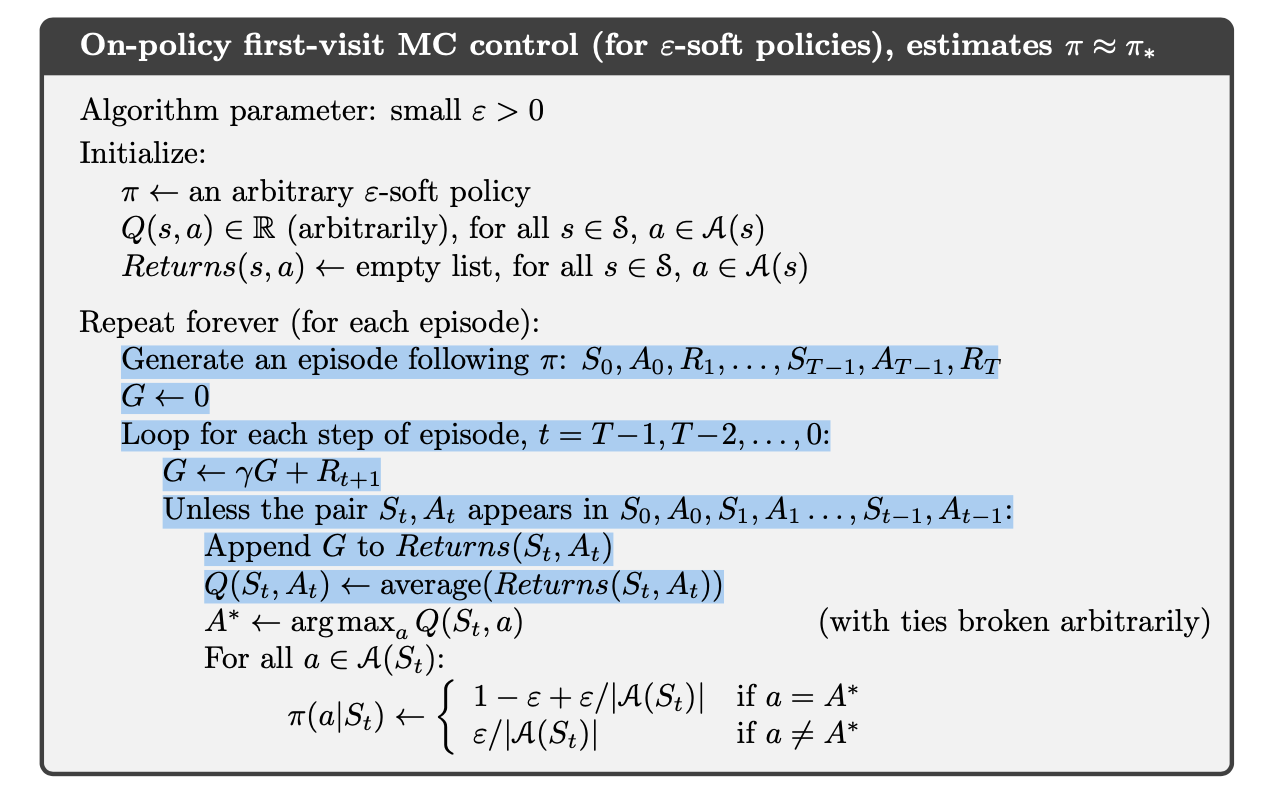
\includegraphics[width=0.75\textwidth]{1.png}
\end{figure}

\subsection*{Sarsa原理}
\begin{figure}[H]
    \centering
    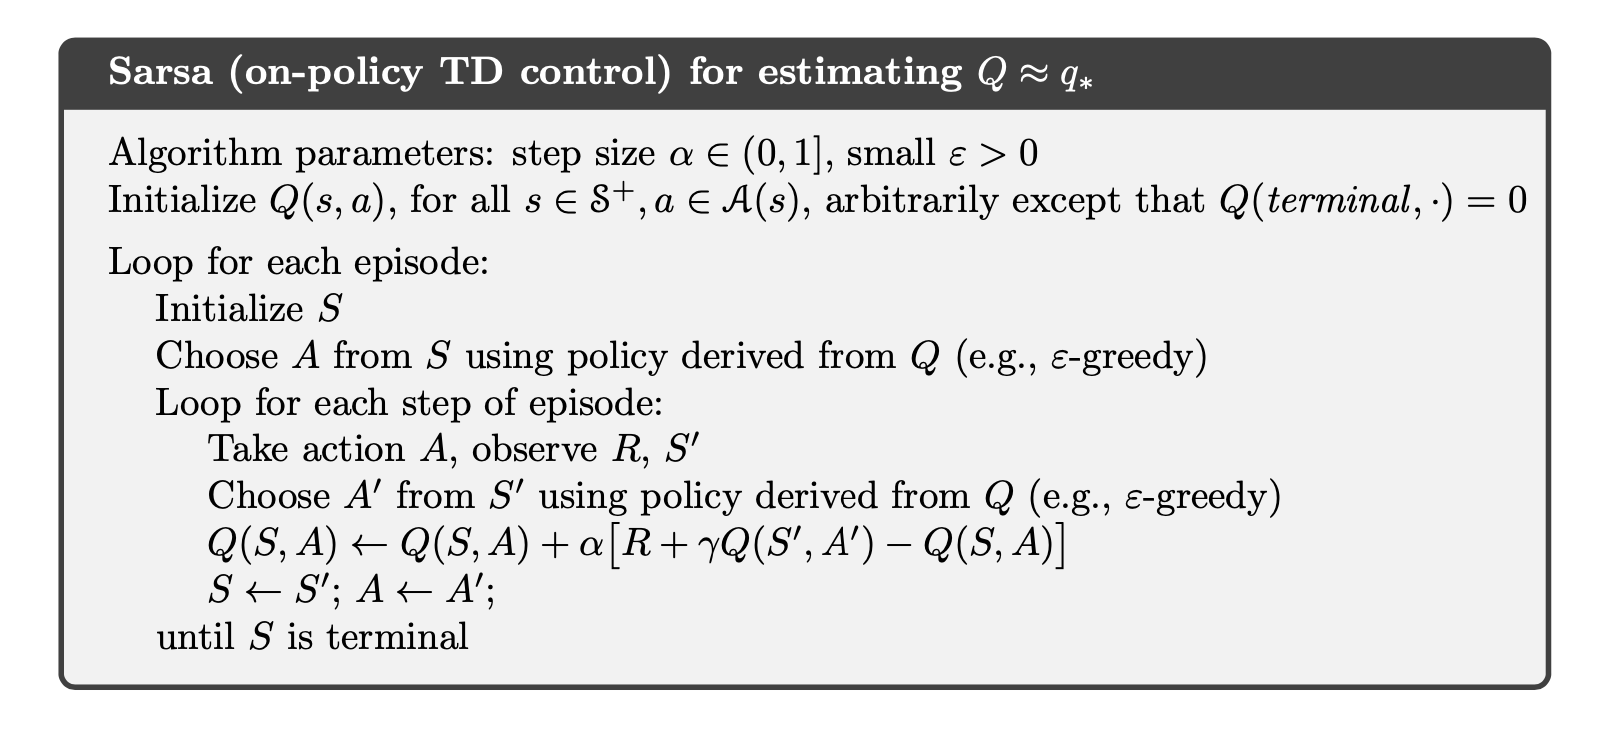
\includegraphics[width=0.75\textwidth]{2.png}
\end{figure}

\subsection*{Q-learning原理}
\begin{figure}[H]
    \centering
    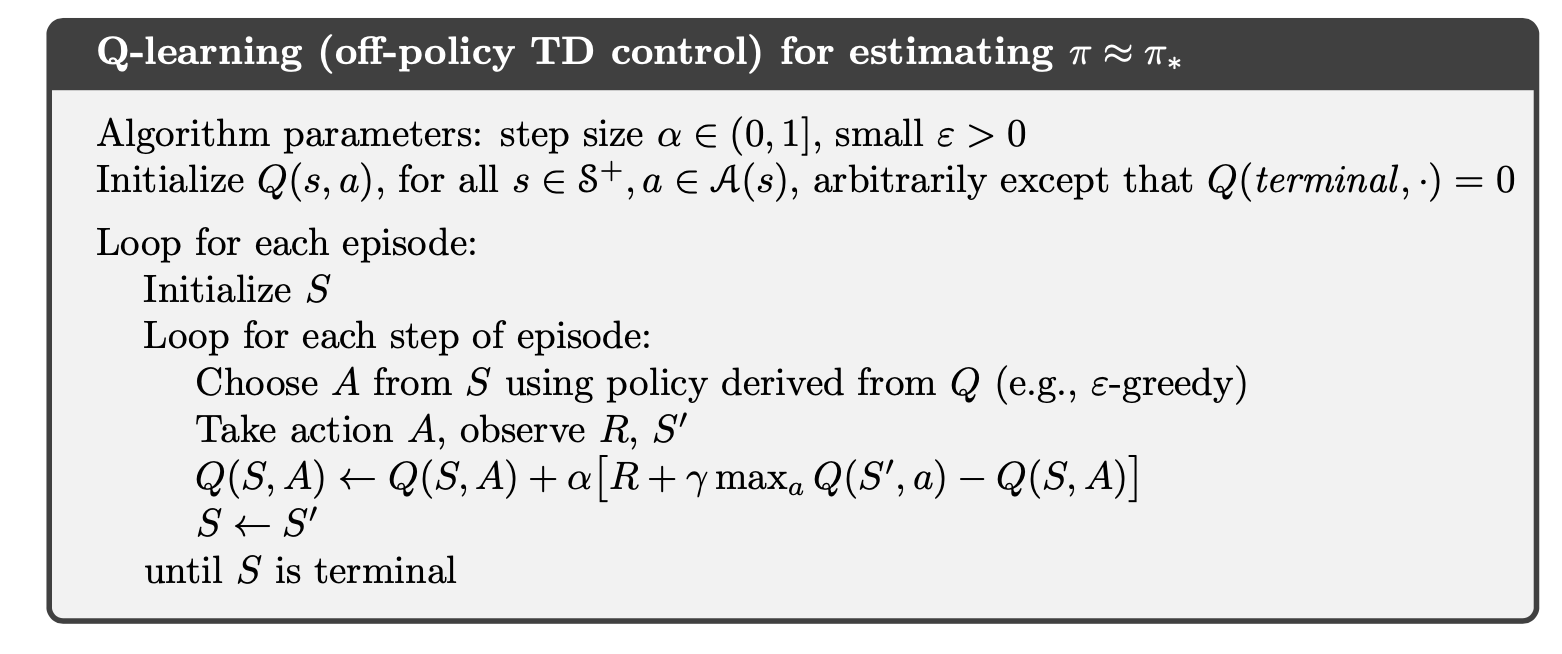
\includegraphics[width=0.75\textwidth]{3.png}
\end{figure}

\section{实验内容}
\subsection*{MC方法实现}
\begin{minted}[breaklines]{python}

# 步骤 1: 生成一个回合。
    # 一个回合是由(状态,动作,奖励)元组组成的数组
episode = []
state = env.reset()
while True:
    # 根据状态选择动作的概率分布
    probs = [0.8, 0.2] if state[0] > 18 else [0.2, 0.8]  # 概率分布
    action = np.random.choice(np.arange(2), p=probs)  # 根据概率选择动作
    next_state, reward, done, info = env.step(action)  # 执行动作,获取下一个状态、奖励等信息
    episode.append((state, action, reward))  # 记录状态、动作和奖励
    state = next_state
    if done:
        break

# 步骤 2: 找出我们在这个回合中访问过的所有(状态,动作)对
states, actions, rewards = zip(*episode)  # 解压回合元组,获取状态、动作和奖励信息

# 步骤 3: 计算所有采样回合中该状态的平均回报
discounts = np.array([discount_factor**i for i in range(len(rewards) + 1)])  # 计算折扣因子
for i, state in enumerate(states):
    # 更新动作值函数
    returns_sum[state][actions[i]] += sum(rewards[i:] * discounts[:-(i + 1)])  # 计算回报总和
    returns_count[state][actions[i]] += 1  # 记录访问次数
    Q[state][actions[i]] = returns_sum[state][actions[i]] / returns_count[state][actions[i]]  # 计算平均值


\end{minted}

\subsection*{Sarsa方法实现}
\begin{minted}[breaklines]{python}

# 步骤 1:执行一步
next_state, reward, done, _ = env.step(action)  # 执行选定的动作,获取下一个状态、奖励等信息
# 步骤 2:选择下一个动作
next_action_probs = policy(next_state)  # 获取下一个状态下的动作概率分布
next_action = np.random.choice(np.arange(len(next_action_probs)), p=next_action_probs)  # 根据概率选择下一个动作
# 更新统计信息
stats.episode_rewards[i_episode] += reward  # 更新回合奖励
stats.episode_lengths[i_episode] = t  # 更新回合长度

# 步骤 3:时序差分更新
td_target = reward + discount_factor * Q[next_state][next_action]  # 计算时序差分目标值
td_delta = td_target - Q[state][action]  # 计算时序差分误差
Q[state][action] += alpha * td_delta  # 更新动作值函数

if done:  # 如果当前回合结束
    break  # 跳出循环,结束回合
    
action = next_action  # 更新当前动作为下一步的动作
state = next_state  # 更新当前状态为下一步的状态


\end{minted}

\subsection*{Q-learning方法实现}
\begin{minted}[breaklines]{python}

# 步骤 1:执行一步
action_probs = policy(state)  # 获取当前状态下的动作概率分布
action = np.random.choice(np.arange(len(action_probs)), p=action_probs)  # 根据概率选择动作
next_state, reward, done, _ = env.step(action)  # 执行选定的动作,获取下一个状态、奖励等信息

# 更新统计信息
stats.episode_rewards[i_episode] += reward  # 更新回合奖励
stats.episode_lengths[i_episode] = t  # 更新回合长度

# 步骤 2:时序差分更新
best_next_action = np.argmax(Q[next_state])  # 选择下一个状态中具有最大动作值的动作
td_target = reward + discount_factor * Q[next_state][best_next_action]  # 计算时序差分目标值
td_delta = td_target - Q[state][action]  # 计算时序差分误差
Q[state][action] += alpha * td_delta  # 更新动作值函数
    
if done:  # 如果当前回合结束
    break  # 跳出循环,结束回合
    
state = next_state  # 更新当前状态为下一步的状态

\end{minted}
\section{实验结果}

\begin{figure}[H]
    \centering
    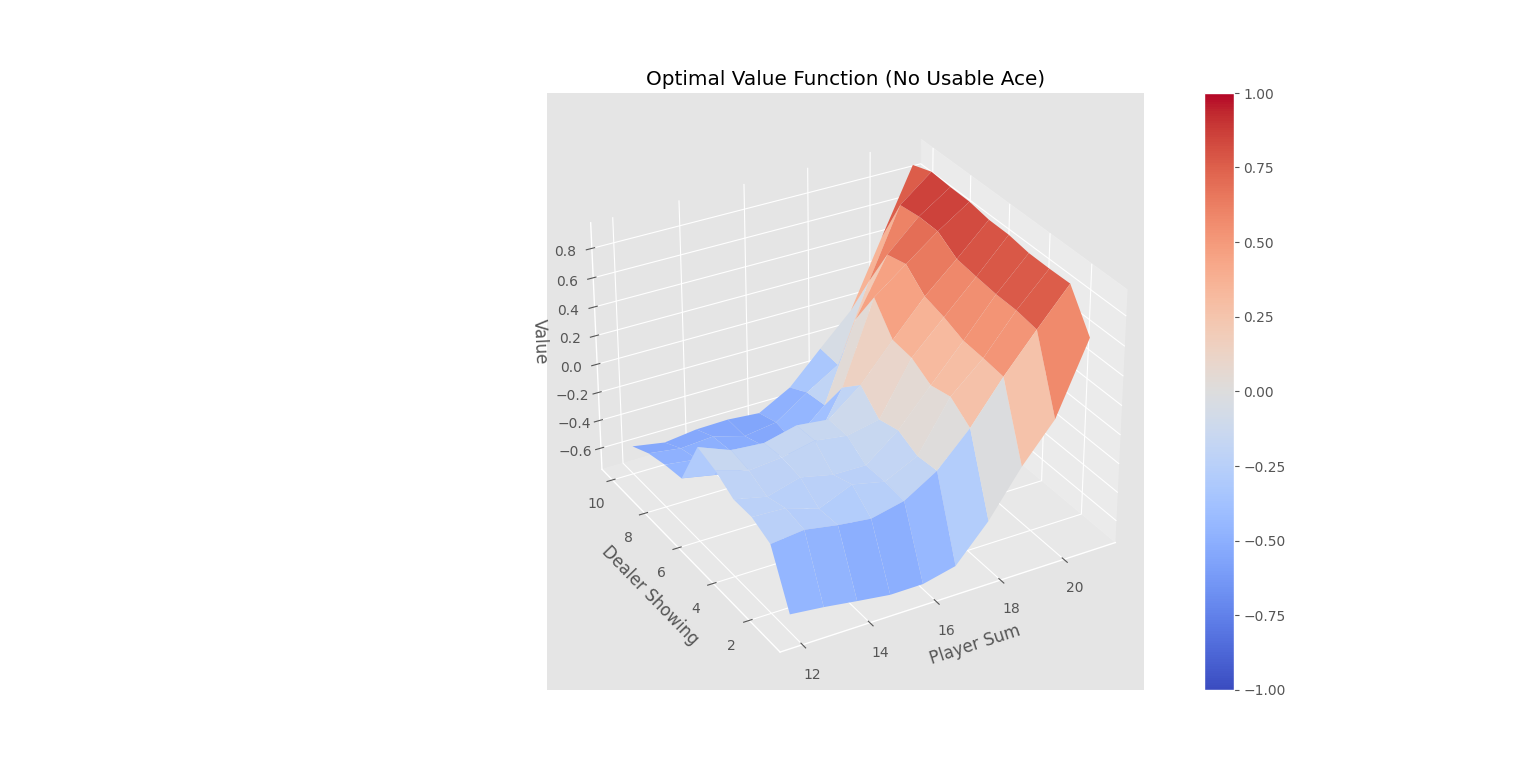
\includegraphics[width=0.4\textwidth]{m1.png}
    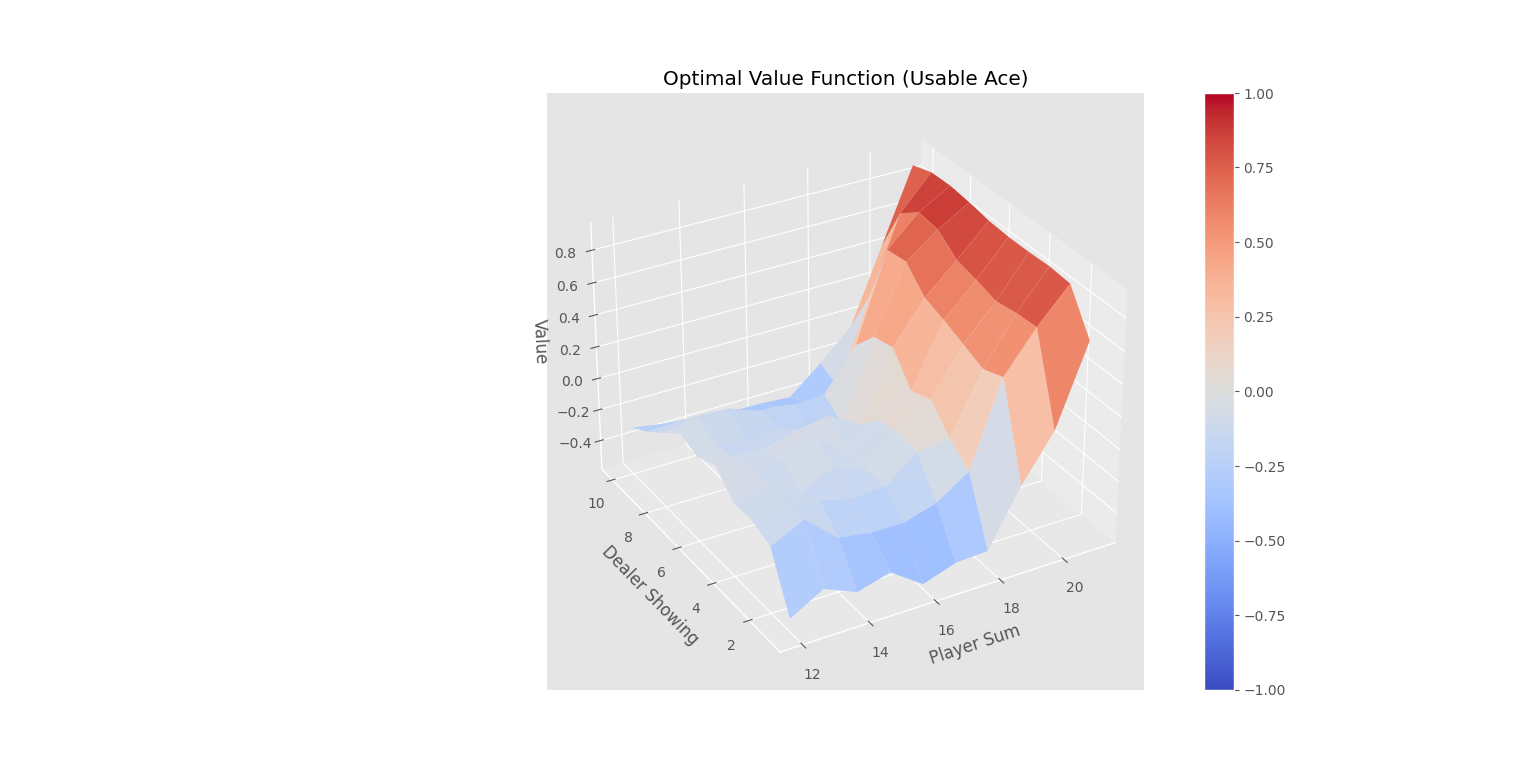
\includegraphics[width=0.4\textwidth]{m2.png}
\end{figure}

经过5000000个episode后,greedy policy依然没有找到最优策略,但是$\epsilon$-greedy policy所找到的最优策略要比单纯的greedy policy好的多。

\begin{figure}[H]
    \centering
    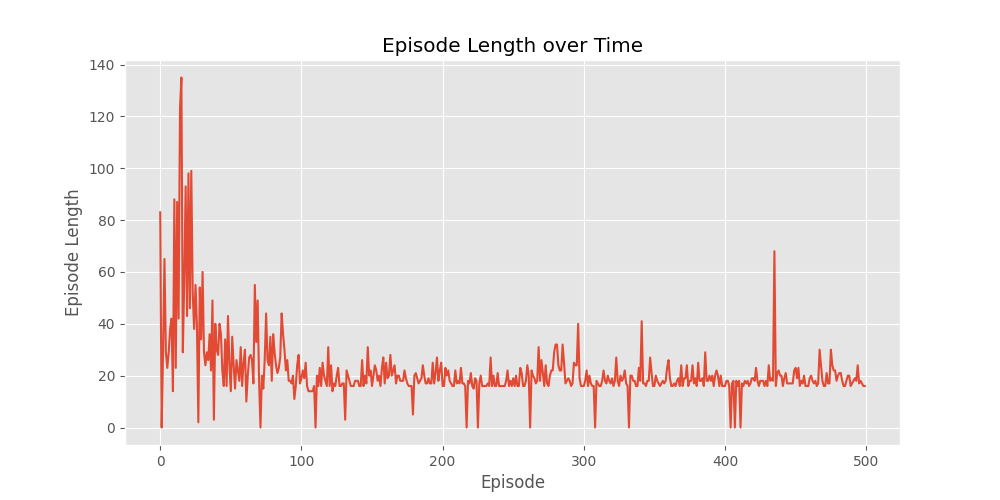
\includegraphics[width=0.3\textwidth]{s1.png}
    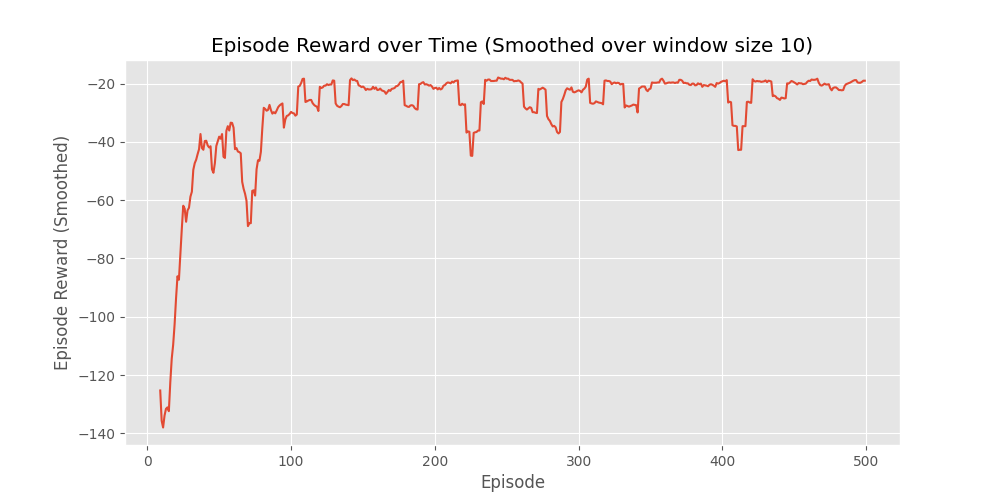
\includegraphics[width=0.3\textwidth]{s2.png}
    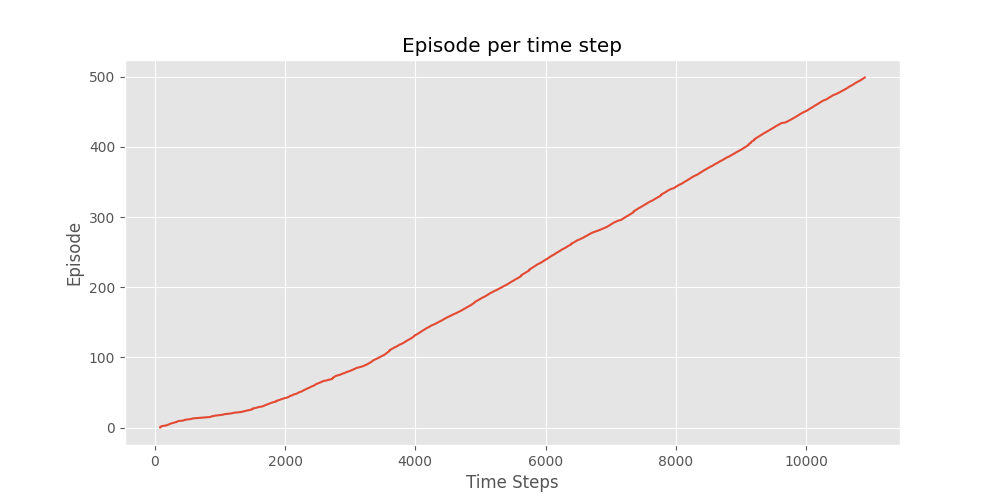
\includegraphics[width=0.3\textwidth]{s3.png}
\end{figure}

\begin{figure}[H]
    \centering
    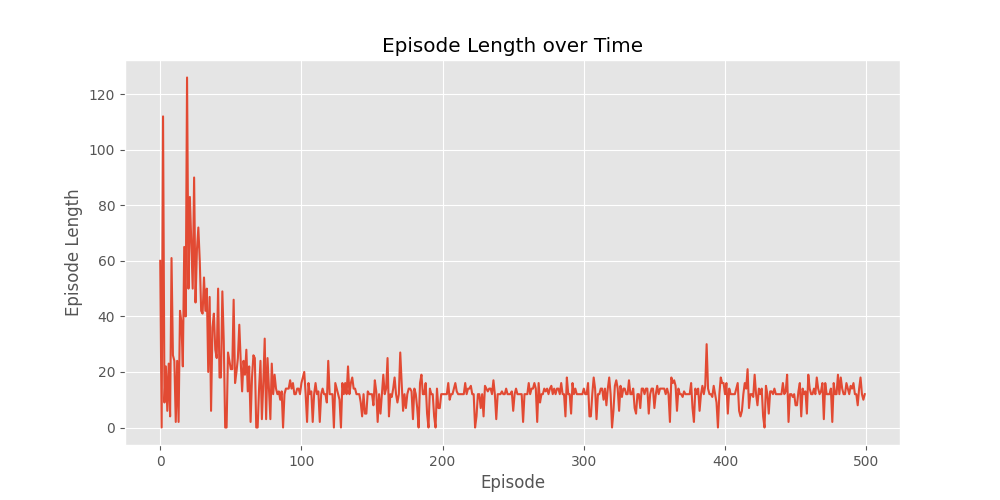
\includegraphics[width=0.3\textwidth]{q1.png}
    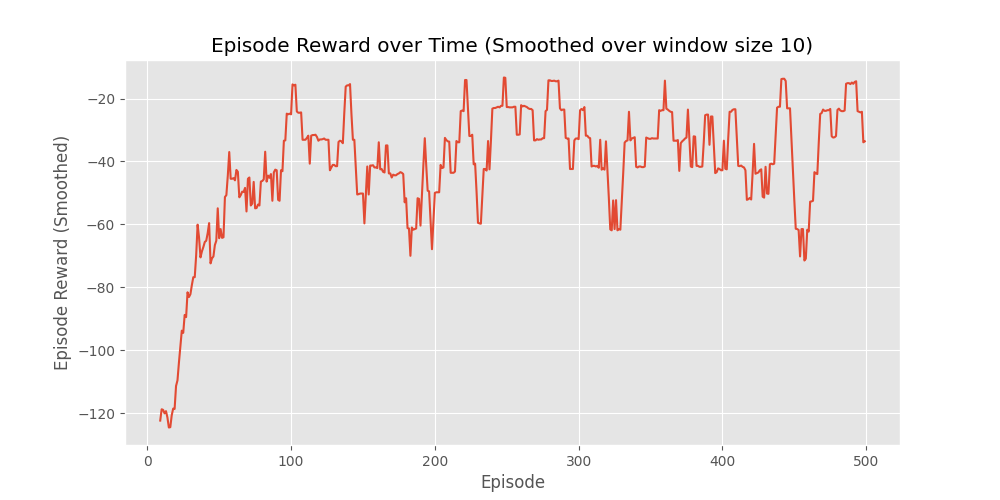
\includegraphics[width=0.3\textwidth]{q2.png}
    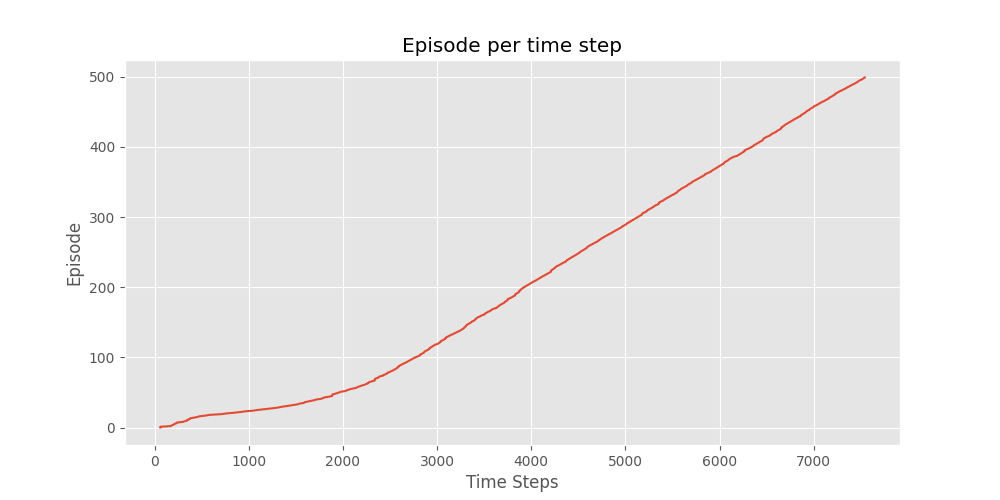
\includegraphics[width=0.3\textwidth]{q3.png}
\end{figure}

用Sarsa和Q-learning两种算法求解最佳策略。Sarsa产生数据的策略和更新Q值的策略相同,即属于on-policy算法;而Q-learning更新Q值的策略为贪婪策略,其产生数据的策略和更新Q值的策略不同,即属于off-policy算法;对于Sarsa算法而言,它的迭代速度较慢,它选择的路径较长但是相对比较安全,因此每次迭代的累积奖励
也比较多,对于Q-leaning而言,它的迭代速度较快,由于它每次迭代选择的是贪婪策略因此它更有可能选择最短路径,不过这样更容易掉入悬崖,因此每次迭代的累积奖励也比较少。
\end{document}